\underline{Nouveau cours du 30/11} \\

\begin{figure}[!h]
    \centering
    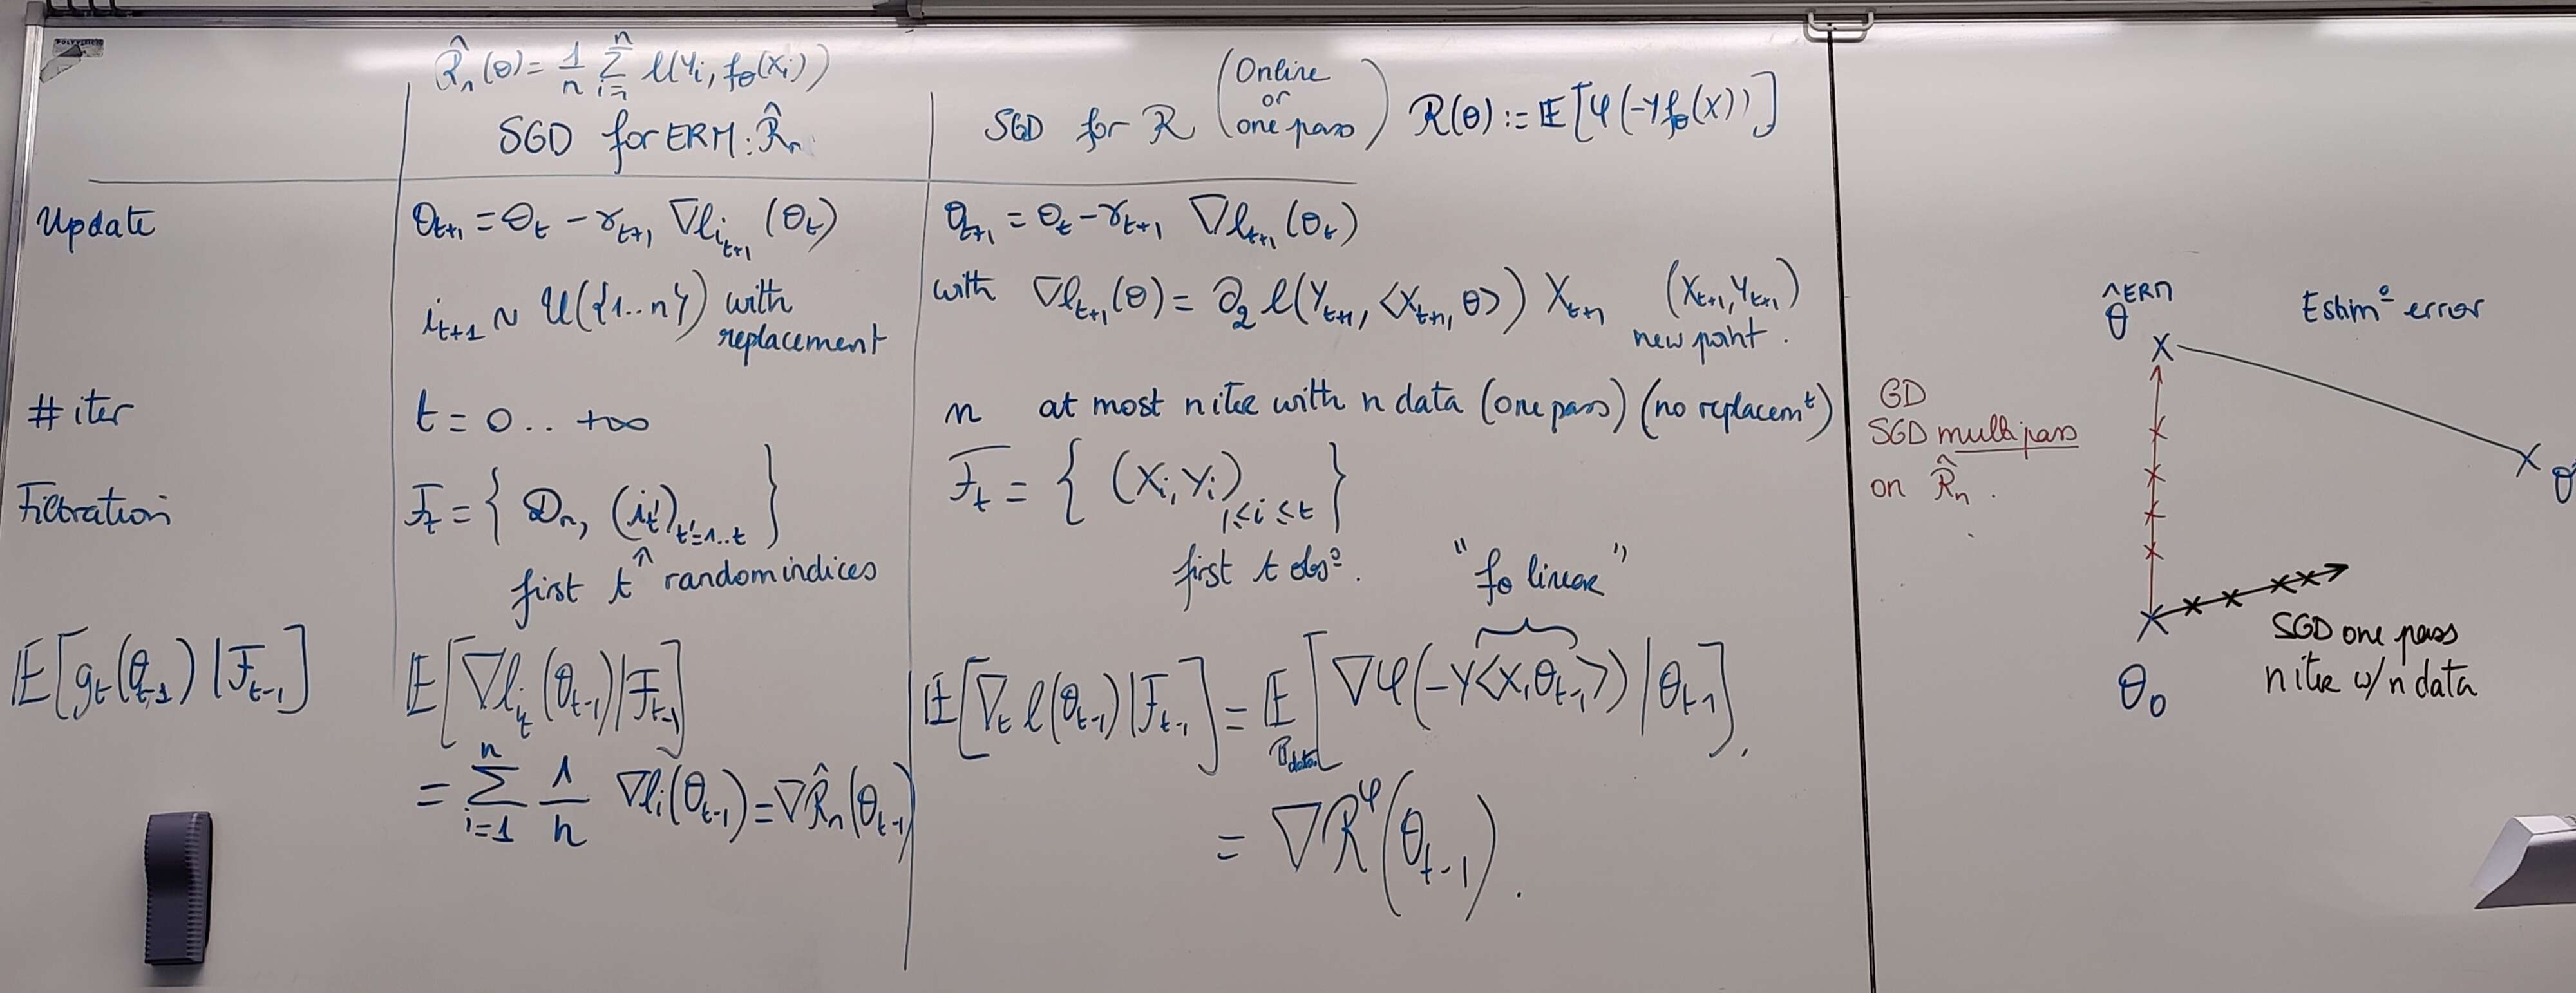
\includegraphics[width=.95\textwidth]{figs/sum_up_SGD_table.jpg}
    \caption{Comparaison between SGD for ERM $\hat{\mathcal{R}}_n$ and SGD for $\mathcal{R}$ }
\end{figure}

\textbf{Averaging} : In the case of strongly cvx fonction \& smooth
\begin{itemize}
    \item SGD with no averaging $ \gamma _t = Ct^{- \alpha }, \alpha =1 $
    \item SGD + averaging $ \gamma _t = C t^\alpha , \frac{1}{2} \leq \alpha \leq 1 $ rate : $ \mathcal{O} (t^{-1} \mu ^{-1} ) $ 
\end{itemize}

=> Averaging help in case of "bad choice" of step size. \\
\textbf{Take-home message} : use $\alpha  = \frac{1}{2}$ + averaging.


\chapter{Stability of learning Algorithm \& generalizations}

\section{Motivation}
\begin{figure}[!h]
    \centering
    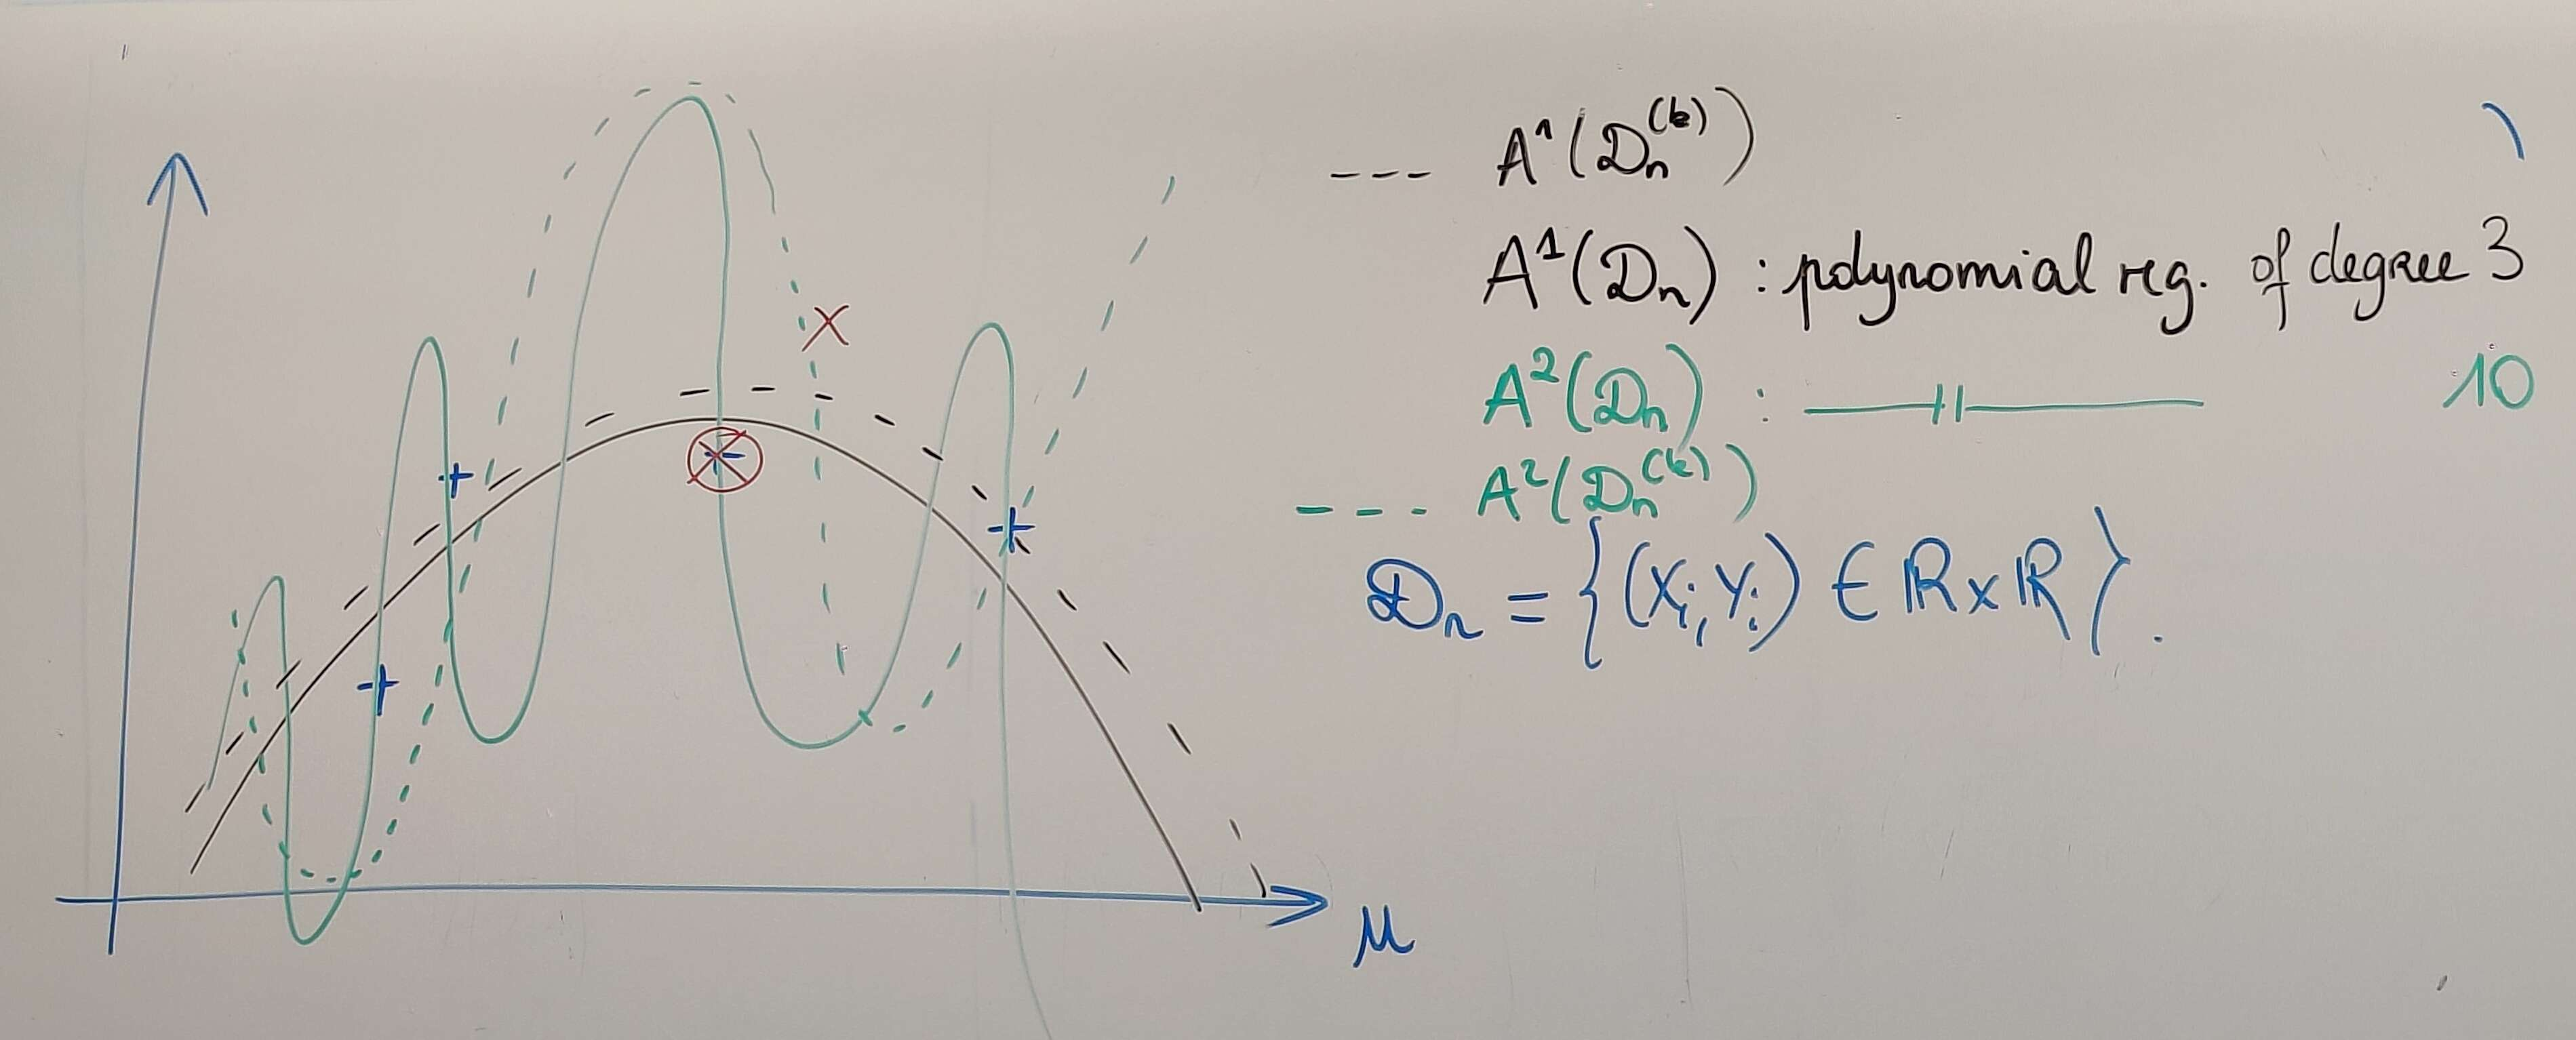
\includegraphics[width=.8\textwidth]{figs/chapter_4_motivation.jpg}
    \caption{Chapter 4: Motivation. The black algorythm seem better (better generalization, less overfitting) }
\end{figure}

\textbf{Generalization} : for a test point $(X, Y)$ of same distrib and $\ind $ of $\mathcal{D}_n$, evaluation of $\mathbb{E}[l(Y, A(\mathcal{D}_n)(X))]$

Another point of view of generalization : compare $ A(\mathcal{D}_n ) $ vs $ A(\mathcal{D}_n^{(k)}) $ where $ \mathcal{D} _n ^{(k)} $ is the training set in which we change the $ k $-th point.

\[
    \mathcal{D}_n^{(k) \leftarrow (X'_{k}, y'_{k} )} = {(X_1, Y_1) ... (X_{k-1}, Y_{k-1}),(x'_{k}, y'_{k}),(X_{k+1}, Y_{k+1}), ... (X_n, Y_n)}
.\]
In the picture  \begin{itemize}
    \item $ A^1 (\mathcal{D}_n) $ is "close" to $ A^1( \mathcal{D }_n ^{(k)}) $ 
    \item $ A^2 (\mathcal{D}_n) $ is very different from $ A^2( \mathcal{D }_n ^{(k)}) $ $\rightarrow A^2$  is unstable.
\end{itemize}
Claim : Stability implies generalization 

\begin{defn}[]
    A learning algo $(A_n)_n$ is a sequence of mapping
    \begin{align*}
        A_n : (\mathcal{X}&, \mathcal{Y})^{\times n} \to \mathcal{C} \\
                &\mathcal{D}_n \mapsto A_n (\mathcal{D}_n ) (\text{ possibly random})
    \end{align*}
    from any number of points into the set $\mathcal{C}$ of classifier.
\end{defn}

\begin{exmp}[1]
    Empirical risk minimizer over $ \Theta  $ is a learning algo 
    \[
        A^{ERM}(\mathcal{D}_n) \equiv \arg \min_{\theta \in \Theta}\hat{\mathcal{R}}_{n, \mathcal{D}_n }(\theta )
    .\]
    
\end{exmp}


\begin{exmp}[This is a \textbf{randomized algo}]
    SGD with T steps and $(\gamma _t)_{t=1...T}$ is a learning algo
    \[
        A^{SGD} \equiv \begin{cases}
            \theta _0 &= 0 \\
            \theta _{t+1} &= \theta _t - \gamma _{t+1} g_{t+1} (\theta _t) \text{ for } t = 0, \dots, T-1 \\
        \end{cases}
    .\]
    where $ g_t (\theta _{t-1} ) $ is the gradient of 
    \[
        \theta  \mapsto l(Y_{i_t} , \left\langle \theta , X_{i_t} \right\rangle ), i_t \sim \mathcal{U}(\{1, \dots, n\})
    .\]
    
\end{exmp}

\begin{defn}[Uniform stability (deterministic algo)]
    Concider a deterministic algo A \\
    A is uniformly stable for $ \beta : \mathbb{N} \to \mathbb{R}_+ $ if for \textbf{any} $\mathcal{D}_n$, for \textbf{any} $k$, for \textbf{any} $(X'_k, Y'_k) \in \mathcal{X} \times \mathcal{Y}$, for any test point $(X_{test}, T_{test}) \in \mathcal{X}, \mathcal{Y}$ 
    \[
        \left| l(Y_{test}, A(\mathcal{D}_n)(X_{test})) - l(Y_{test}, A(\mathcal{D}_n^{(k) \leftarrow (X'_{k}, Y'_{k} )})(X_{test})) \right| \leq \beta (n)
    .\]
    
\end{defn}

\begin{defn}[Uniform stability (randomized algo)]
    Concider a randomized algo A \\
    A is uniformly stable for $ \beta_{av} : \mathbb{N} \to \mathbb{R}_+ $ if for \textbf{any} $\mathcal{D}_n$, for \textbf{any} $k$, for \textbf{any} $(X'_k, Y'_k) \in \mathcal{X} \times \mathcal{Y}$, for any test point $(X_{test}, T_{test}) \in \mathcal{X}, \mathcal{Y}$ 
    \[
        \mathbb{E}[\left| l(Y_{test}, A(\mathcal{D}_n)(X_{test})) - l(Y_{test}, A(\mathcal{D}_n^{(k) \leftarrow (X'_{k}, Y'_{k} )})(X_{test})) \right|] \leq \beta_{av} (n)
    .\]
    Thi only random thing is the algo
\end{defn}

\begin{note}[]
    We could extend thses definitions to EXPECTED stability (kind of a less stronger version) : for $ (X_i, Y_i)_{i=1} ^n, (X_k^\prime , Y_k^\prime ), (X_{test}, Y_{test}) \sim \mathbb{P}_{data}^{\otimes (n+2)} $ 
\end{note}

\paragraph*{Ref} : \begin{itemize}
    \item Stability introduced in Bousquet \& Elisseeff (2002)
    \item Re-introduced by HArdt, Recht, Singer "Train faster, generalize bettter" (2016)
    \item Widely used since then
\end{itemize}

\begin{note}[]
    Related to algorithm sensibility, privacy-preserving algo with DP (differential privacy) \\
    \[
        (\epsilon , \delta ) \text{-DP} : \forall S, \mathbb{P}(A(\mathcal{D}_n) \in S) \leq (1+\epsilon ) \mathbb{P}(A(\mathcal{D}_n^{(k)}) \in S) + \delta 
    .\]
    $\leadsto $ Aurélien Bellet, french expert in Monpelier.
\end{note}

\section{Stability implies generalization}


\textbf{Warning}: A stupid algo A such that $ \forall \mathcal{D}_n, A(\mathcal{D_n}) = \theta _0 \ind \mathcal{D}_n $ is $ \beta $-stable for $ \beta = 0 $. \\

\textbf{Intuition}: the generalization ability should be controlled by : 1. Stability term ; 2. Data-fitting term. \\

\begin{lem}[]
    Call $ \theta ^\star  = \arg \min_{\theta  \in  \Theta } \mathcal{R}(\theta )$  and $\theta ^{ERM} = \arg \min_{\theta  \in  \Theta} \hat{\mathcal{R}}_{n, \mathcal{D}_n}(\theta )$
\begin{align*}
    \mathbb{E}[ \mathcal{R} (A (\mathcal{D}_n )) - \mathcal{R} (\theta ^\star )] \leq &\mathbb{E}[ \underbrace{\mathcal{R} (A (\mathcal{D}_n )) - \hat{\mathcal{R}} _{n, \mathcal{D}_n} (A (\mathcal{D}_n ))}_{\text{Difference between generalisation / empirical errors } \approx \text{Stability}}     ] \\
    & + \underbrace{\mathbb{E}[ \hat{\mathcal{R}}_{n, \mathcal{D}_n} (A (\mathcal{D}_n)) - \hat{\mathcal{R}}_{n ,\mathcal{D}_n} ( \hat{\theta }^{ERN })]}_{\text{optim error} \leadsto \text{ data fitting term}}
\end{align*}
\end{lem}

\begin{note}[]
    For any predictor $\theta _0 \ind \mathcal{D}_n $ 
    \[
        \mathcal{R}(\theta _0) = \mathbb{E}[\hat{\mathcal{R}}_{n, \mathcal{D}_n}(\theta_0 )]
    .\]
    
\end{note}

\begin{proof}[Proof:]
    \begin{align*}
        \mathcal{R}(A(\mathcal{D}_n)) - \mathcal{R}(\theta ^\star ) &= \mathcal{R}(A(\mathcal{D}_n)) - \hat{\mathcal{R}} _{n, \mathcal{D}_n} (A (\mathcal{D}_n )) \\
        &+ \hat{\mathcal{R}} _{n, \mathcal{D}_n} (A (\mathcal{D}_n )) - \hat{\mathcal{R}} _{n, \mathcal{D}_n} (\hat{\theta }^{ERM}) \\
        &+ \hat{\mathcal{R}} _{n, \mathcal{D}_n} (\hat{\theta }^{ERM}) - \hat{\mathcal{R}} _{n, \mathcal{D}_n} (\hat{\theta }^{\star }) \quad \textcolor{red}{\leq 0 \text{ since } \hat{\theta }^{ERM} \in \arg \min _{\Theta } \hat{\mathcal{R}} _{n, \mathcal{D}_n}}\\
        &+ \hat{\mathcal{R}} _{n, \mathcal{D}_n} (\hat{\theta }^{\star }) - \mathcal{R}(\theta ^\star ) \\
    \end{align*}
    And 
    \begin{align*}
        \mathbb{E}[\mathcal{R}(A(\mathcal{D}_n)) - \mathcal{R}(\theta ^\star )] &= \mathbb{E}[\mathcal{R}(A(\mathcal{D}_n)) - \hat{\mathcal{R}} _{n, \mathcal{D}_n} (A (\mathcal{D}_n )) ] \\
        &+ \mathbb{E}[\hat{\mathcal{R}} _{n, \mathcal{D}_n} (A (\mathcal{D}_n )) - \hat{\mathcal{R}} _{n, \mathcal{D}_n} (\hat{\theta }^{ERM}) ] \\
        &+ \mathbb{E}[\hat{\mathcal{R}} _{n, \mathcal{D}_n} (\hat{\theta }^{ERM}) - \hat{\mathcal{R}} _{n, \mathcal{D}_n} (\hat{\theta }^{\star }) ] \\
        &+ \mathbb{E}[\hat{\mathcal{R}} _{n, \mathcal{D}_n} (\hat{\theta }^{\star }) - \mathcal{R}(\theta ^\star )] \quad \textcolor{red}{=0 \text{ since } \theta ^\star \ind \mathcal{D}_n} \\
    \end{align*}
\end{proof}

\begin{note}[]
    For example 1, $ A(\mathcal{D}_n) \equiv \hat{\theta }^{ERN} $, Lemma 22 gives 
    \[
        \mathbb{E}[ \mathcal{R} (A (\mathcal{D}_n))] - \mathcal{R} (\theta ^\star ) \leq  \mathbb{E}[ \mathcal{R}(A(\mathcal{D}_n)) - \hat{\mathcal{R} } _{n, \mathcal{D}_n} ( A(\mathcal{D}_n)) ]
    .\]
    the optim error vanishes
\end{note}

\begin{thm}[Stability $\rightarrow$ Generalization]
    If A is a learning algo which is $ \beta  $-uniformly stable then 
    \[
        \mathbb{E}[ \mathcal{R}(A(\mathcal{D}_n)) - \hat{\mathcal{R}}_{n,\mathcal{D}_n}] \leq \beta (n)
    .\]
\end{thm}
\begin{proof}[Proof:]
    Reminder \begin{itemize}
        \item $ \mathcal{R} (A(\mathcal{D}_n)) = \mathbb{E}_{(X,Y) \sim p}[ l(Y, A(\mathcal{D}_n)) | \mathcal{D}_n] $ 
        \item $ \mathbb{E}_{\mathcal{D}_n} [ \mathcal{R}(A (\mathcal{D}_n))] $ 
        \item $ \hat{\mathcal{R}}_{n, \mathcal{D}_n} (A(\mathcal{D}_n)) = \frac{1}{n} \sum_{i=1}^{n } l (Y_i, A(\mathcal{D}_n) (X_i)) $ 
        \item $ \mathbb{E}_{\mathcal{D}_n} [ \hat{\mathcal{R}}_{n, \mathcal{D}_n}(A (\mathcal{D}_n))] $ 
    \end{itemize}
    Observe that for any $ k \in \{1, \dots, n\} $ 
    \begin{align*}
        \mathbb{E} [\mathcal{R}(A(\mathcal{D}_n))]
            &= \mathbb{E}_{ \mathcal{D}_n \sim p^{\otimes n} ,, \ind (X,Y)\sim p} [ l(Y, A (\mathcal{D}_n) (X)) ] \\
            &= \mathbb{E}_{ \mathcal{D}_n \sim p^{\otimes n} ,, \ind (X,Y)\sim p} [ l(Y_k, A(\mathcal{D}_n^{(k)}) (X_k))]
    \end{align*}
    Since $ ( (X_1, Y_1), \dots, (X_k, Y_k), \dots, (X_n, Y_n), (X,Y) ) = ^{\text{dist}} ( (X_1, Y_1), \dots, (X, Y) \dots, (X_n, Y_n), (X_k,Y_k) )$ 

    Therefore
    \begin{align*}
        \mathbb{E} [\mathcal{R}(A(\mathcal{D}_n)) - \hat{\mathcal{R}}_{n, \mathcal{D}_n} (A(\mathcal{D}_n))] 
            &= \mathbb{E}[ \frac{1}{n} \sum_{k=1}^{n} ( \mathcal{R} (A ( \mathcal{D}_n) ) - l ( Y_k, A(\mathcal{D}_n) (X_k)))] \\
            &= \frac{1}{n} \sum_{k=1 }^{n} \mathbb{E}[ \underbrace{l( Y_k, A(\mathcal{D}_n ^{(k) (X,Y) })(X_k) ) -l (Y_k , A(\mathcal{D}_n) (X_k))}_{ \leq \beta (n) \text{ by stability assumption}} ] \\
            &\leq \beta (n)
    \end{align*}
\end{proof}

\textbf{CCL} : 
\begin{itemize}
    \item (BEFORE) $ gen \leq \underbrace{\text{state rate}}_{\text{Worst } \hat{\mathcal{R}}_n - \mathcal{R} \text{ on } \theta \in \Theta ( \text{ Uniform bounds})}$ + optim rate \\
    \item (NOW) $ gen \leq \underbrace{stab}_{\text{This term is algo-dependent}} $ + optimization.
\end{itemize}


\section{Computing the stability $\beta $ for ERM with a strongly cvx risk} 

\textbf{Hypothesis} : $\theta \mapsto \hat{\mathcal{R}}_ {n, \mathcal{D}_n}(\theta )$ is $\mu $-strongly cvx \\
\textbf{Remark}: Is the relaxed risk strongly cvx in ML? \\
When $F \in  \mathcal{C}^2$, $\forall \theta,  \nabla ^2 F(\theta ) \succcurlyeq \mu$ Id. i.e $\lambda_{\text{MIN}}(\nabla ^2 F(\theta )) \geq \mu $ \\
When $ \hat{\mathcal{R}}_n (\theta ) = \frac{1}{n} \sum_{i=1}^{n} \varphi (-X_i^T \theta Y_i), Y_i \in \{\pm 1\}, Y_i^2 = 1 $ then \begin{align*}
    \nabla \hat{\mathcal{R }}_n (\theta ) &= \frac{1}{n }\sum_{i=1 }^{n } ( -\varphi ^\prime  (-X_i^T \theta Y_i ) Y_i X_i) \\
    \nabla ^2 \hat{\mathcal{R }}_n (\theta ) &= \frac{1}{n } \sum_{i=1 }^{n } \varphi ^{\prime \prime } (-X_i^T \theta Y_i ) \underbrace{X_i X_i^T}_{\in \mathbb{R}^{d \times d}}
\end{align*}
If $\varphi $ is $\mu$-strongly cvx from $\mathbb{R}$ to $\mathbb{R}$, the $\forall u, \varphi ''(u) \geq \mu  $ and $\nabla ^2 \hat{\mathcal{R}_n}(\theta ) \succcurlyeq \mu  \frac{1}{n} \sum_{i=1}^{n} X_i X_i^T$ i.e. $ \lambda _{\text{MIN}}(\nabla ^2 \hat{\mathcal{R}_n}(\theta )) \geq \mu \lambda _{\text{MIN}}(\frac{1}{n} \sum_{i=1}^{n} X_i X_i^T)  $\\
And $\frac{1}{n} \sum_{i=1}^{n} X_i X_i^T \to_{n \to + \infty } \text{Cov}(X)$ by the LLN if ($(X_i)_i$ centered.

The strong convexity of $ \hat{\mathcal{R }}_n  $ is linked to the lowest eigenvalue of $ Cov(X) $. It can be small (!!) and if $ d > n  $ then $ \lambda _{\text{MIN}} ( \frac{1 }{n } \sum_{i=1 }^{n } X_i X_i^T ) = 0 $ almost surely.

Finally strong convexity is not always true or $\mu $ can be small. Note that regularization can bring strong convexity 
\[
    \min _{\theta } \hat{\mathcal{R}}(\theta ) + \frac{\mu}{2 } \left\| \theta  \right\|^2_2 
.\]
The ridge regularized risk is $\mu $ strongly cvx.


\begin{thm}[]
    Let $ \hat{\theta }^{ORN} = \arg \min _{\theta \in \mathbb{R}^d} \hat{\mathcal{R}}_{n,\mathcal{D}_n} (\theta )$ with $ \hat{\mathcal{R}}_{n,\mathcal{D}_n} $  $ \mu  $-strongly convex. \\
    Assume that the loss function $ l  $ is $ \beta  $-Lipschitz w.r.t. it's second argument i.e.
    \[
        \forall y, z, z^\prime , \left| l(y,z) - l(y,z^\prime ) \right| \leq \beta \left| z - z^\prime  \right| 
    .\]
    Assume that $ \left\| X \right\| _2 \leq \mathcal{R} $ a.s. \\
    Then, the ERM algo $ A(\mathcal{D}_n) \equiv \hat{\theta }^{ERM} $   is $ \frac{4 \beta ^2 R^2}{\mu n} $ uniformly stable.\\ 
    $\rightarrow$ \textbf{Good:} this is a fast rate !! [see Srebro, Sridahran, Shalev-shwartz]
\end{thm}

\begin{proof}[Proof:]
    \begin{enumerate}
        \item By strong convexity, $\hat{\mathcal{R}}_{n, \mathcal{D}_n}(\theta ) - \hat{\mathcal{R}}_{n, \mathcal{D}_n}(\overbrace{A(\mathcal{D}_n)}^{\hat{\theta }^{ERM}}) \geq  \frac{\mu }{2} \left\| \theta  - A(\mathcal{D}_n) \right\|^2_2 $ \\
            Let $ k \in \{1, \dots, n\} $, apply this inequation to $ \theta = A(\mathcal{D}_n ^{(k)}) $ then $ \hat{\mathcal{R}}_{n, \mathcal{D}_n} (A(\mathcal{D}_n)) - \hat{\mathcal{R}}_{n,\mathcal{D}_n} (A(\mathcal{D}_n)) \geq \frac{\mu }{2} \left\| A(\mathcal{D}_n ^{(k)}) - A(\mathcal{D}_n)  \right\| _2 ^2 $ 
        \item \begin{align*}
            \hat{\mathcal{R}}_{n, \mathcal{D}_n} (A (\mathcal{D}_n^{(k)} )) - \hat{\mathcal{R}}_{n, \mathcal{D}_n} (A (  \mathcal{D}_n )) 
                &= \frac{1}{n } \sum_{i=1, i \neq k}^{n} l(Y_i, A(\mathcal{D}_n ) (X_i)) - l(Y_i, A(\mathcal{D}_n )(X_i)) &\text{ (L1)}\\
                &+ \frac{1}{n} [ l(Y'_k, A(\mathcal{D}_n^{(k)})(X'_k)) - l(Y'_k, A(\mathcal{D}_n)(X'_k))] &\text{ (L2)}\\
                &- \frac{1}{n} [ l(Y'_k, A(\mathcal{D}_n^{(k)})(X'_k)) - l(Y'_k, A(\mathcal{D}_n)(X'_k))] &\text{ (L3)}\\
                &+ \frac{1}{n} [ l(Y_k, A(\mathcal{D}_n^{(k)})(X_k) )- l(Y_k, A(\mathcal{D}_n)(X_k))] &\text{ (L4)}\\
        \end{align*}
    \end{enumerate}
    \begin{itemize}
        \item L1 + L2 $\rightarrow \hat{\mathcal{R}}_ {n, \mathcal{D}_n^{(k)}}(A(\mathcal{D}_n^{(k)})) - \hat{\mathcal{R}}_ {n, \mathcal{D}_n^{(k)}}(A(\mathcal{D}_n^)) \leq 0 $ a.s 
        \item L3 \& L4 $\leq \frac{1}{n}.B.\left| A(\mathcal{D}_n^{(k)})(X_k) - A(\mathcal{D}_n)(X_k) \right| \leq \frac{B}{n} \left| A(\mathcal{D}_n^{(k)})(X_k) - A(\mathcal{D}_n) \right|_2 \underbrace{\left| Xk \right| 2}_{\leq R} $ (with $A(\mathcal{D}_n)(X_k) = A(\mathcal{D}_n)^T X_k$
        \item 1 \& 2 $\rightarrow$ \begin{align*}
            \frac{\mu }{2} \left\| A(\mathcal{D}_n ^{(k)}) - A(\mathcal{D}_n) \right\| _2 ^2 &\leq_{a.s.} \underbrace{2}_{\text{from L3+L4}} \frac{B.R}{n } \left\| A(\mathcal{D}_n ^{(k)}) - A(\mathcal{D}_n) \right\| _2 \underbrace{\left\| X_k \right\| _2}_{\leq R} \\
            \left\| A(\mathcal{D}_n ^{(k)}) - A(\mathcal{D}_n) \right\| _2 &\leq \frac{4BR}{\mu n} \\
            \Rightarrow \forall (x,y), \left| l(y, A(\mathcal{D}_n ^{(k)})) - l(y, A(\mathcal{D}_n)(x)) \right| &\leq \frac{4B^2 RR^2}{\mu n}
        \end{align*} 
    \end{itemize}
    Finaly, A is $ \beta  $-univormly stable. 
\end{proof}

\begin{note}[]
    We have provent a stronger condition than stability, i.e. $ A(\mathcal{D}_n) $ is close to $ A(\mathcal{D}_n ^{(k)}) $ in Euclidien norm 
\end{note}

\section{Stability of SGD ()}
\textbf{Algo} 
\begin{align*}
                &\theta _0 (\gamma _t)_{t=1} ^T \\
                &\forall 0 \leq t \leq T-1, \theta _{t+1} = \theta _t - \gamma _t g_{t+1} (\theta _t) \\
    \text{with }&g_{t+1}(\theta ) = \nabla _\theta l(Y_{i_{t+1}}, X_{i_{t+1}}^T \theta ) (\text{ linear predictors )} \\
                &i_{t+1} \sim \mathcal{U}(\{1, \dots, n\})
\end{align*}

\textbf{Question} studying the stability of SGD requires to understand $A(\mathcal{D}_n)$ vs $A(\mathcal{D}_n)^{(k)}$
\begin{figure}[!h]
    \centering
    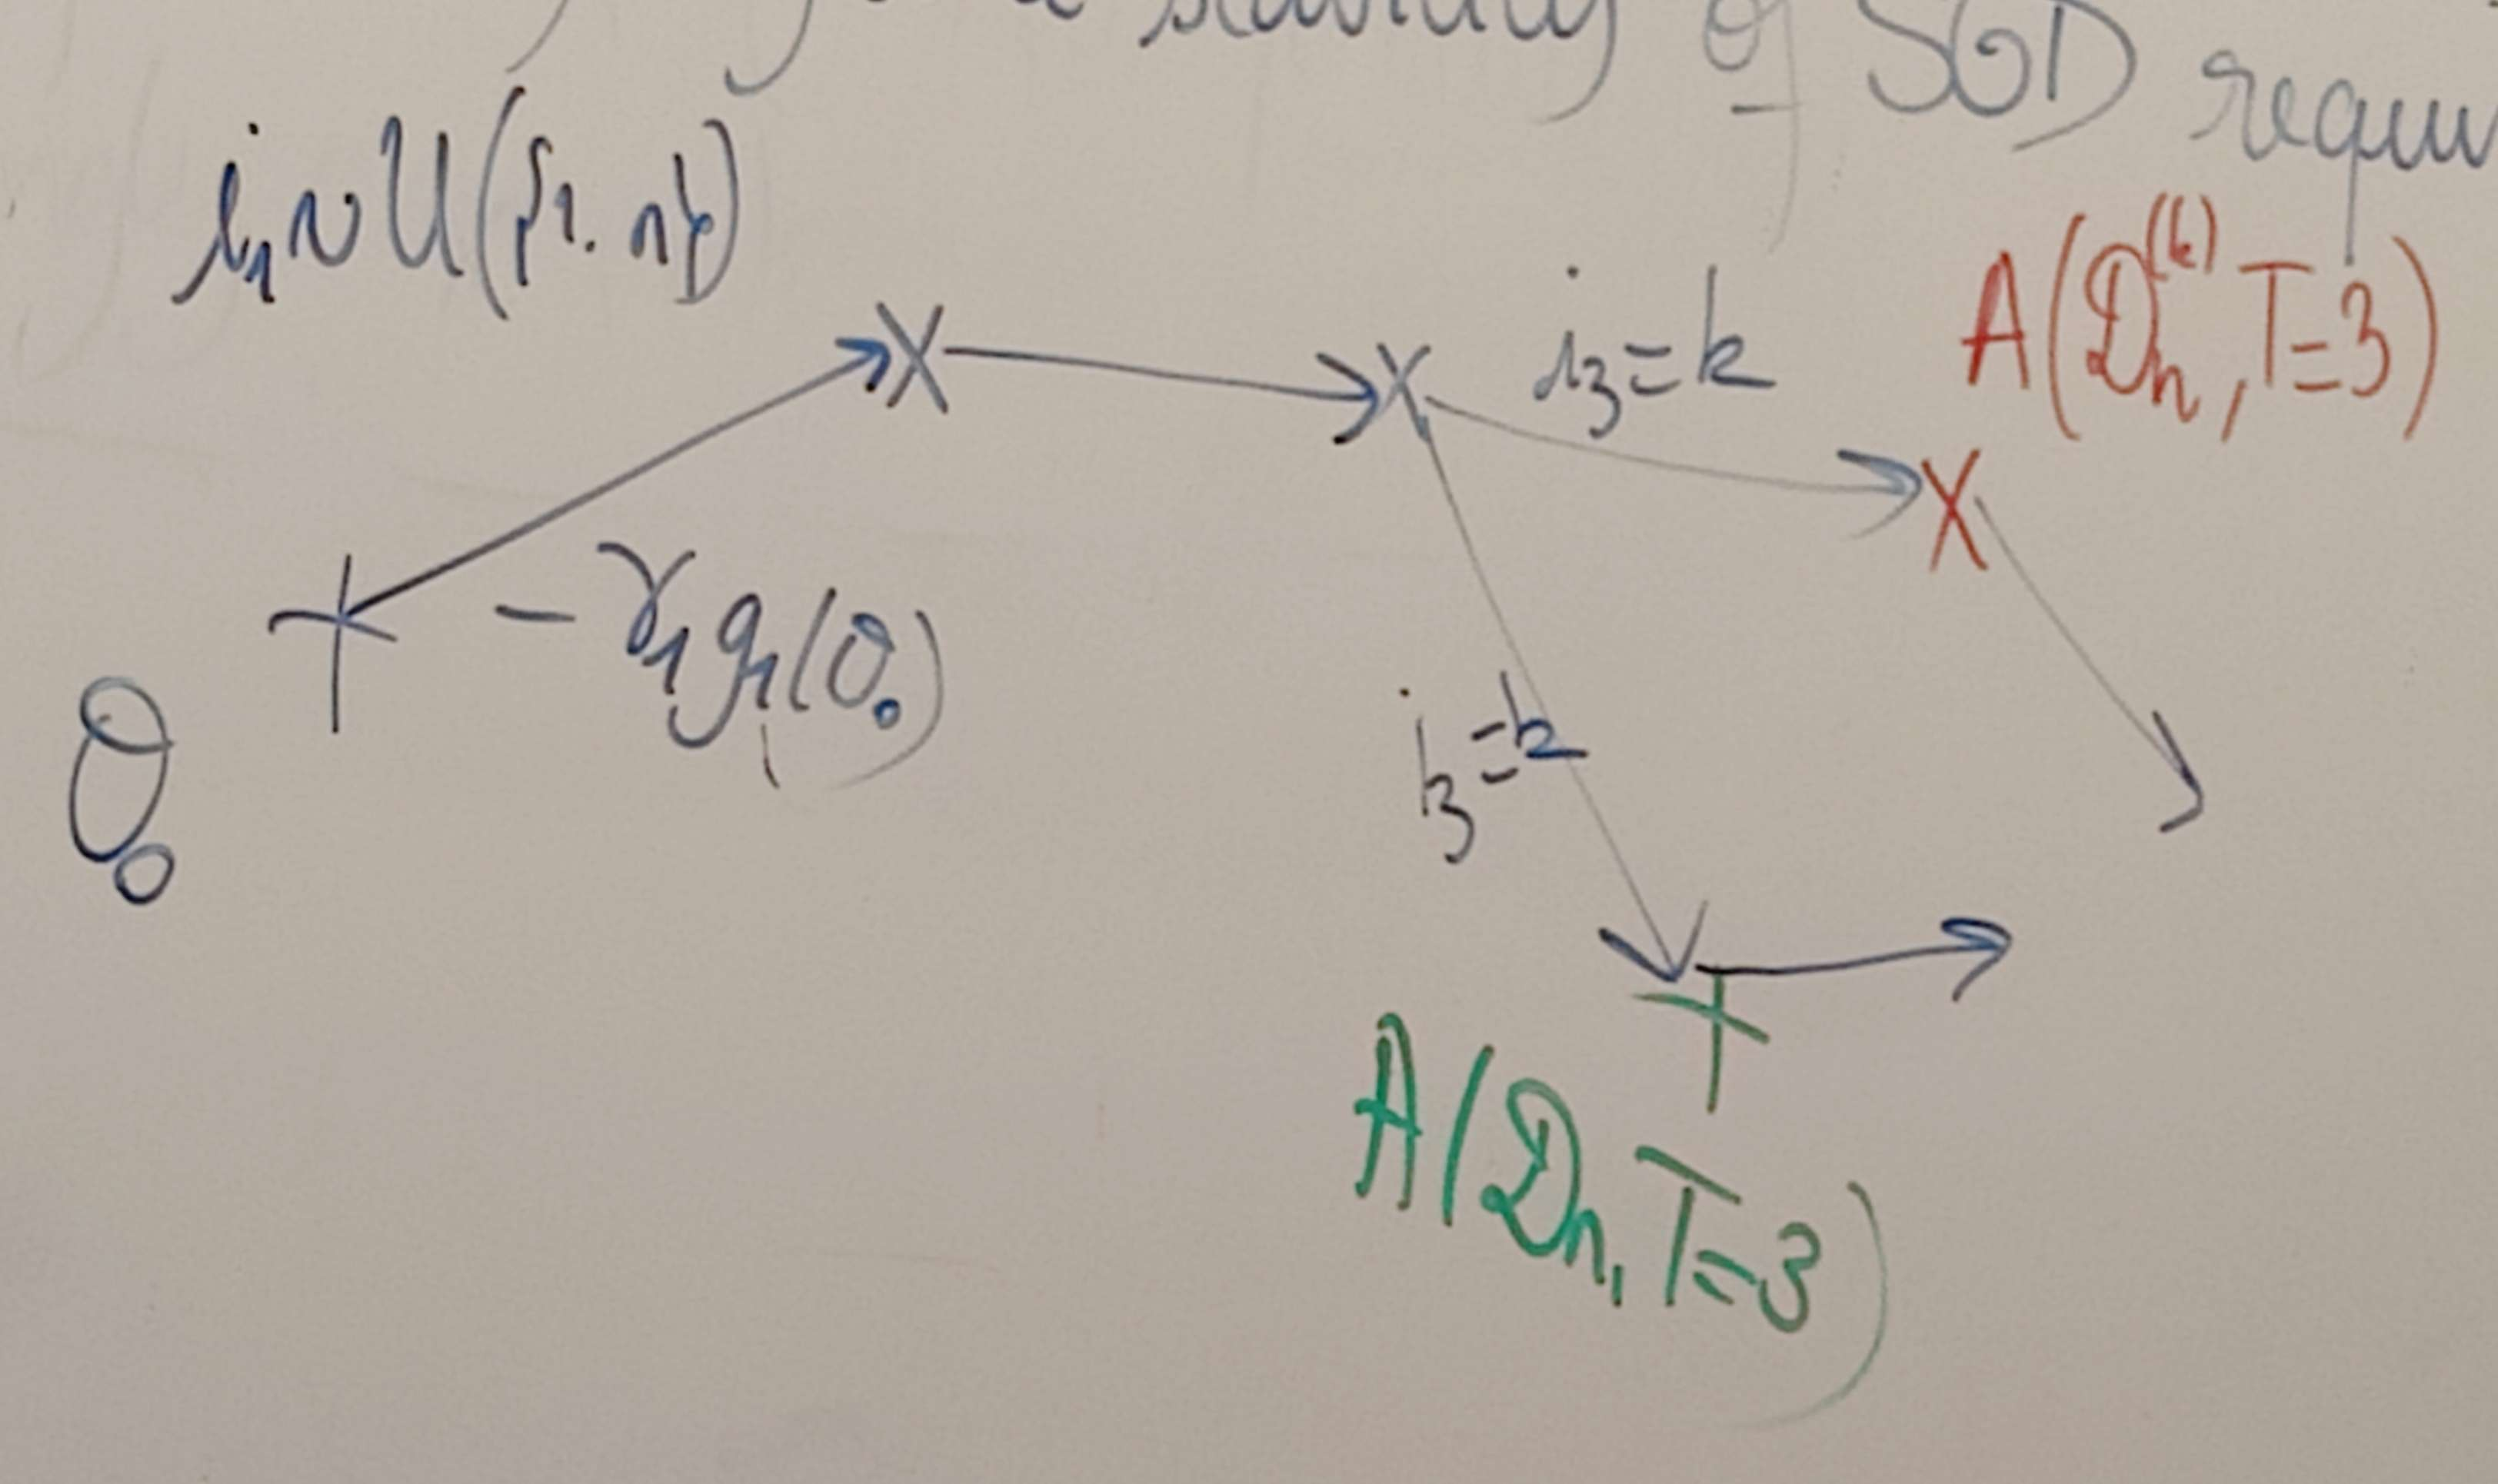
\includegraphics[width=.65\textwidth]{figs/graph.jpg}
    \caption{Difference between $A(\mathcal{D}_n)$ vs $A(\mathcal{D}_n)^{(k)}$}
\end{figure}

\textbf{goal} Control $A(\mathcal{D}_n, T_{\text{steps}}) - A(\mathcal{D}_n^{(k)}, T_{\text{steps}})$ where
\begin{itemize}
    \item for most of the steps with $\mathbb{P} = \frac{n-1}{n}$,I use the same gradients $(g_{i_t})$, $i_t \neq k$ (at different points)
    \item for some steps with $\mathbb{P} = \frac{1}{n}$, I use $g_k$ for $A(\mathcal{D}_n)$ and $g'_k$ for $A(\mathcal{D}_n^{(k)})$
\end{itemize}


\textbf{Key argument: } for any convex and $ L $-smooth $ F $, then $ \forall \theta , \eta  $ 
\begin{align*}
    \left\| \theta - \gamma \nabla F(\theta ) - \eta  + \gamma \nabla F(\eta )  \right\| _2 ^2 
        &= \left\| \theta - \eta  \right\| _2 ^2 - 2 \gamma \left\langle \theta - \eta , \nabla F(\theta ) - \nabla F(\eta ) \right\rangle + \gamma ^2 \underbrace{\left\| \nabla F(\theta ) - \nabla F(\eta ) \right\| _2 ^2}_{\leq L \left\langle \nabla F(\theta ) - \nabla F(\eta ) , \theta - \eta  \right\rangle \text{ cocoercivite}} \\
        &\leq \left\| \theta - \eta  \right\| ^2 - \underbrace{2 \gamma (1 - \frac{\gamma L }{2 }) }_{\geq 0 \text{ if } \gamma L \leq 2 } \underbrace{\left\langle \theta  - \eta , \nabla F(\theta ) - \nabla F (\eta )  \right\rangle }_{\geq 0 \text{ when } F \text{ cvx}} \\
        (\text{ if } \gamma L \leq 2) & \leq \left\| \theta  - \eta  \right\| ^2 
\end{align*}

With stong convexity, we would get $\leq  (1 - 2 \gamma \mu (1- \frac{\gamma L}{2})) \left| \theta - \eta  \right|^2 $

\begin{thm}[]
    Consider $ A \equiv  $ Algo 2, i.e. SGD with $ T $ steps \& step size $ (\gamma _t)_{t=1,\dots,T} $. \\
    Assume that $ \forall k \in \{1, \dots, n\}, \psi : \theta \mapsto l (Y_k, X_k^T \theta ) $ is convex, L-Smooth, BR Lipschitz (which is ok for $ l $ B-Lip \& $ \left\| X  \right\| \leq R  $ a.s. ) \\
    Then A is uniformly stable with $ \beta (n) = \frac{2 B^2 R^2 \sum_{t=1 }^{T } \gamma _t }{n} $ 
\end{thm}

